\documentclass[paper=a4, fontsize=11pt]{scrartcl} % A4 paper and 11pt font size

%----------------------------------------------------------------------------------------
%	PACKAGES
%----------------------------------------------------------------------------------------
\usepackage[T1]{fontenc} % Use 8-bit encoding that has 256 glyphs
\usepackage{fourier} % Use the Adobe Utopia font for the document - comment this line to return to the LaTeX default
\usepackage[english]{babel} % English language/hyphenation
\usepackage{amsmath,amsfonts,amsthm} % Math packages
\usepackage{sectsty} % Allows customizing section commands
\usepackage{fancyhdr} % Custom headers and footers
\usepackage{xcolor} % Allows 0-255 RGB values
\usepackage{tabularx, outlines, framed, varwidth, enumitem, graphicx, listings, color, qtree, float, subcaption, newfloat}
\usepackage[left=0.5in, right=0.5in, top=3in, bottom=.25in]{geometry}
\geometry{}

%----------------------------------------------------------------------------------------
%	SET CUSTOMIZATIONS AND FUNCTIONS
%----------------------------------------------------------------------------------------
\sectionfont{\centering \normalfont\scshape} % Make all sections centered, the default font and small caps
\pagestyle{fancyplain} % Makes all pages in the document conform to the custom headers and footers
\fancyhead{} % No page header - if you want one, create it in the same way as the footers below
\fancyfoot[L]{} % Empty left footer
\fancyfoot[C]{} % Empty center footer
\fancyfoot[R]{\thepage} % Page numbering for right footer
\renewcommand{\headrulewidth}{0pt} % Remove header underlines
\renewcommand{\footrulewidth}{0pt} % Remove footer underlines
\setlength{\headheight}{0pt} % Customize the height of the header

\DeclareFloatingEnvironment[fileext=lod]{diagram}

\numberwithin{equation}{section} % Number equations within sections (i.e. 1.1, 1.2, 2.1, 2.2 instead of 1, 2, 3, 4)
\numberwithin{figure}{section} % Number figures within sections (i.e. 1.1, 1.2, 2.1, 2.2 instead of 1, 2, 3, 4)
\numberwithin{table}{section} % Number tables within sections (i.e. 1.1, 1.2, 2.1, 2.2 instead of 1, 2, 3, 4)

\graphicspath{{./figures/}}
%\setlength\parindent{0pt} % Removes all indentation from paragraphs - comment this line for an assignment with lots of text

\makeatletter
	\newcommand*\variableheghtrulefill[1][.4\p@]
	{%
		\leavevmode
		\leaders \hrule \@height #1\relax \hfill
		\null
	}
\makeatother

\definecolor{solBase03}{RGB}{000,043,054}
\definecolor{solBase02}{RGB}{007,054,066}
\definecolor{solBase01}{RGB}{088,110,117}
\definecolor{solBase00}{RGB}{101,123,131}
\definecolor{solBase0}{RGB}{131,148,150}
\definecolor{solBase1}{RGB}{147,161,161}
\definecolor{solBase2}{RGB}{238,232,213}
\definecolor{solBase3}{RGB}{253,246,227}
\definecolor{solYellow}{RGB}{181,137,000}
\definecolor{solOrange}{RGB}{203,075,022}
\definecolor{solRed}{RGB}{220,050,047}
\definecolor{solMagenta}{RGB}{211,054,130}
\definecolor{solViolet}{RGB}{108,113,196}
\definecolor{solBlue}{RGB}{038,139,210}
\definecolor{solCyan}{RGB}{042,161,152}
\definecolor{solGreen}{RGB}{133,153,000}

\lstdefinestyle{mystyle}{
	% To Match
	sensitive=true,	
	%
	% Add border
	frame=lines,
	%
	% Add Margin
	xleftmargin=\parindent,
	%
	% Put extra space under caption
    belowcaptionskip=1\baselineskip,
    %
    % Colors:
	backgroundcolor=\color{solBase3},
    basicstyle=\color{solBase00}\footnotesize,
    keywordstyle=\color{solCyan},
    commentstyle=\color{solBase1},
    stringstyle=\color{solBlue},
    numberstyle=\color{solViolet},
    identifierstyle=\color{solBase00},
    %
    % Formatting Options
    breakatwhitespace=false,
    breaklines=true, % break long lines
    captionpos=b,
    keepspaces=true,
    numbers=left,
    numbersep=5pt,
    showspaces=false,
    showstringspaces=false,
    showtabs=false,
    tabsize=4
}

\lstdefinestyle{smallstyle}{
	% To Match
	sensitive=true,	
	%
	% Add border
	frame=lines,
	%
	% Add Margin
	xleftmargin=\parindent,
	%
	% Put extra space under caption
    belowcaptionskip=1\baselineskip,
    %
    % Colors:
	backgroundcolor=\color{solBase3},
    basicstyle=\color{solBase00}\scriptsize,
    keywordstyle=\color{solCyan},
    commentstyle=\color{solBase1},
    stringstyle=\color{solBlue},
    numberstyle=\color{solViolet},
    identifierstyle=\color{solBase00},
    %
    % Formatting Options
    breakatwhitespace=false,
    breaklines=false, % break long lines
    captionpos=b,
    keepspaces=true,
    numbers=left,
    numbersep=5pt,
    showspaces=false,
    showstringspaces=false,
    showtabs=false,
    tabsize=2
}
 
\lstset{style=mystyle}

%----------------------------------------------------------------------------------------
%	USEFUL COMMANDS
%----------------------------------------------------------------------------------------
%	\makebox[\textwidth][c]{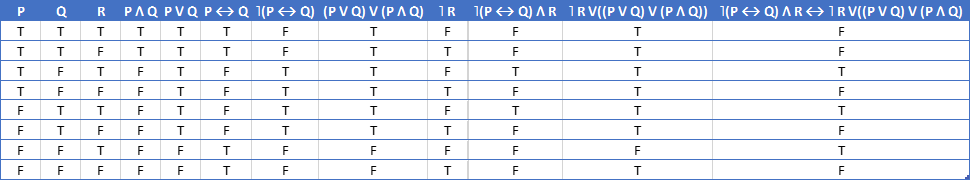
\includegraphics[width=.9\paperwidth]{p2-table}}

%	\newgeometry{top=.75in, bottom=.75in, left=.25in,right=.25in}
%	\newgeometry{top=.75in, bottom=.75in, left=1.25in,right=1.25in}

%	\lstinputlisting[firstline=0, language=C, style=mystyle]{CMPSC360_Homework.cpp}

%\Tree
%	[.<root> [.<left> ][.<middle> ][.<right> ]]

%----------------------------------------------------------------------------------------
%	TITLE SECTION
%----------------------------------------------------------------------------------------

\newcommand{\horrule}[1]{\rule{\linewidth}{#1}} % Create horizontal rule command with 1 argument of height
% \title{Template: Homework 1}
\title{	
\normalfont \normalsize 
%\textsc{Rutgers University, Real Analysis I} \\ [25pt] % Your university, school and/or department name(s)
\horrule{0.5pt} \\[0.4cm] % Thin top horizontal rule
\huge STAT 461: Homework 4 \\ % The assignment title
\horrule{2pt} \\[0.5cm] % Thick bottom horizontal rule
}

\author{\textbf{\underline{Name:}}Kyle Salitrik | \textit{\textbf{\underline{ID\#:}} 997543474} | \textit{\textbf{\underline{PSU ID:}} kps168}} % Your name

\date{\normalsize\today} % Today's date or a custom date

\begin{document}

\maketitle % Print the title

%----------------------------------------------------------------------------------------
%	PROBLEM 1
%----------------------------------------------------------------------------------------
\newgeometry{top=.75in, bottom=.75in, left=1.25in,right=1.25in}
\section*{\variableheghtrulefill[.25ex]\quad Problem 1 \quad\variableheghtrulefill[.25ex]}
\subsection*{a)}
This model is estimable where: $b_1 = b_2 = 1; b_3 = -2$
\begin{flalign*}
\sum_{n=1}^{3} b_i (\mu + \tau_i) & = 1(\mu + \tau_1) + 1(\mu + \tau_2) - 2(\mu + \tau_3)& \\
& = 2\mu - 2\mu + \tau_1 + \tau_2 - 2\tau_3& \\
& =  \tau_1 + \tau_2 - 2\tau_3 &\\
\sum_{n=1}^{3} b_i \overline{Y}_i & = \overline{Y}_1 + \overline{Y}_2 - 2 \overline{Y}_3 &
\end{flalign*}

\subsection*{b)}
This model is estimable where: $b_1 = b_2 = 0; b_3 = 1$
\begin{flalign*}
\sum_{n=1}^{3} b_i (\mu + \tau_i) & = 0(\mu + \tau_1) + 0(\mu + \tau_2) + 1(\mu + \tau_3)& \\
& = \mu + \tau_3 &\\
\sum_{n=1}^{3} b_i \overline{Y}_i & = 0\overline{Y}_1 + 0\overline{Y}_2 + 1\overline{Y}_3 & \\
& = \overline{Y}_3 &
\end{flalign*}

\subsection*{c)}
This model is not estimable for any real values of $b_i$

\subsection*{d)}
This model is estimable where: $b_1 = b_2 = b_3 = \frac{1}{3}$
\begin{flalign*}
\sum_{n=1}^{3} b_i (\mu + \tau_i) & = \frac{1}{3}(\mu + \tau_1) + \frac{1}{3}(\mu + \tau_2) + \frac{1}{3}(\mu + \tau_3)& \\
& = 3 * \frac{1}{3}\mu + \frac{1}{3}\tau_1 + \frac{1}{3}\tau_2 + \frac{1}{3}\tau_3 &\\
& = \mu + \frac{1}{3}(\tau_1 + \tau_2 + \tau_3) &\\
\sum_{n=1}^{3} b_i \overline{Y}_i & = \frac{1}{3}\overline{Y}_1 + \frac{1}{3}\overline{Y}_2 + \frac{1}{3}\overline{Y}_3 & 
\end{flalign*}

%----------------------------------------------------------------------------------------
%	PROBLEM 2
%----------------------------------------------------------------------------------------
\section*{\variableheghtrulefill[.25ex]\quad Problem 2 \quad\variableheghtrulefill[.25ex]}
\subsection*{a)}
\begin{flalign*}
Y_{it} & = \mu + \tau_i + \epsilon_{it}; \quad i = 1,2,3; \quad t = 1,2,3,4 &\\
\epsilon_{it} &\overset{iid}{\sim} N\left(0,\sigma^2\right) &
\end{flalign*}
1 = Regular
2 = Deodorant
3 = Moisturizing

\subsection*{b)}
For future calculations:
\begin{flalign*}
\overline{Y_i} & = \overline{Y} + \hat{\tau}_i & \\
\hat{\tau}_i & = \overline{Y_i} - \overline{Y} & \\
\overline{Y} & = \frac{1}{12} (-.3-.1-.14+.40+2.63+2.61+2.41+3.15+1.86+2.03+2.26+1.82) = 1.5525\bar{3}& \\
\overline{Y_1} & = \frac{1}{4}(-.3-.1-.14+.40) = -0.035 & \\
\overline{Y_2} & = \frac{1}{4}(2.63+2.61+2.41+3.15) = 2.7 & \\
\overline{Y_3} & = \frac{1}{4}(1.86+2.03+2.26+1.82) = 1.9925 & \\
\hat{\tau}_1 & = \overline{Y_1} - \overline{Y} = -0.035 - 1.5525\bar{3} \approx -1.5875 & \\
\hat{\tau}_2 & = \overline{Y_2} - \overline{Y} = 2.7 - 1.5525\bar{3} \approx 1.475 & \\
\hat{\tau}_3 & = \overline{Y_3} - \overline{Y} = 1.9925 - 1.5525\bar{3} \approx 0.44 & \\
\sum_{n=1}^{3} b_i \overline{Y}_i & = b_1\overline{Y}_1 + b_2\overline{Y}_2 + b_3 \overline{Y}_3 & \\
\sum_{n=1}^{3} b_i \overline{Y}_i & =  -0.035 b_1 + 2.7 b_2 + 1.9925 b_3 &
\end{flalign*}

The LSE for a bar of Deodorant Soap is where: $b_1 = b_3 = 0; \quad b_2 = 1$
\begin{flalign*}
\sum_{n=1}^{3} b_i \overline{Y}_i & =  -0.035 * 0 + 2.7 *1 + 1.9925 * 0& \\
&= 2.7&
\end{flalign*}


\subsection*{c)}
This model is estimable where: $b_1 = 1; b_2 = b_3 = - \frac{1}{2}$
\begin{flalign*}
\sum_{n=1}^{3} b_i (\mu + \tau_i) & = 1(\mu + \tau_1) - \frac{1}{2}(\mu + \tau_2) - \frac{1}{2}(\mu + \tau_3)& \\
& = \mu - 2\left(\frac{1}{2}\mu\right) + \tau_1 - \frac{1}{2}\tau_2 - \frac{1}{2}\tau_3& \\
& =  \tau_1 -\frac{1}{2}(\tau_2 + \tau_3) &\\
\sum_{n=1}^{3} b_i \overline{Y}_i & = \overline{Y}_1 -\frac{1}{2}\overline{Y}_2 - \frac{1}{2}\overline{Y}_3 & \\
& = -0.035 - \frac{1}{2}(2.7 + 1.9925) = -2.38125 &
\end{flalign*}


\subsection*{d)}
\lstinputlisting[language=R]{listings/q2-d.txt}

%----------------------------------------------------------------------------------------
%	PROBLEM 3
%----------------------------------------------------------------------------------------
\section*{\variableheghtrulefill[.25ex]\quad Problem 3 \quad\variableheghtrulefill[.25ex]}
\subsection*{a)}
	\makebox[\textwidth][c]{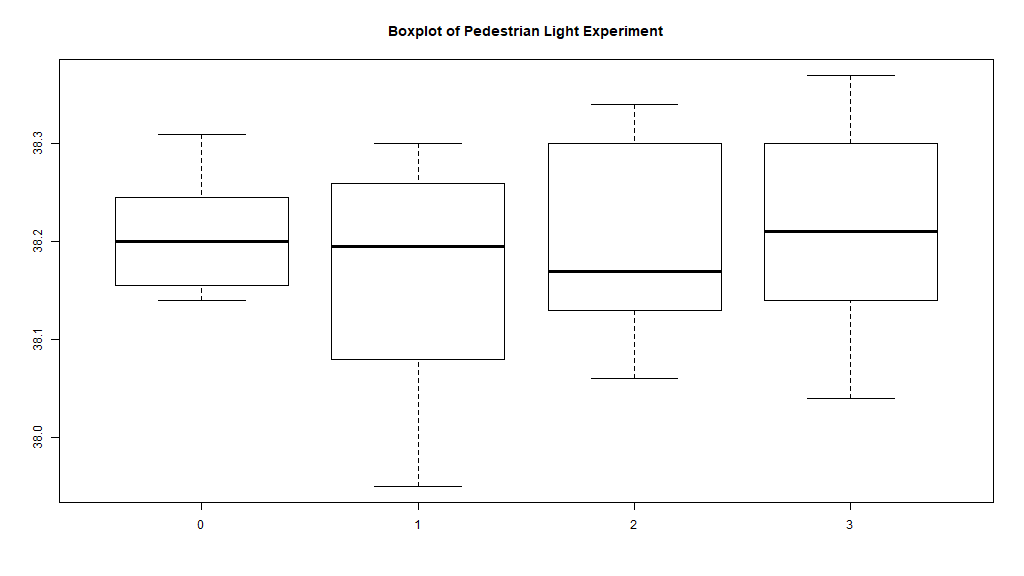
\includegraphics[width=.9\paperwidth]{p3.png}}

\subsection*{b)}
\begin{flalign*}
Y_{it} & = \mu + \tau_i + \epsilon_{it}; \quad i = 0,1,2,3; \quad t = 1,\dots ,r_i &\\
r_1 & = 7, r_1 = r_2 = 10, r_3 = 5 &\\
\epsilon_{it} &\overset{iid}{\sim} N\left(0,\sigma^2\right) &
\end{flalign*}

\subsection*{c)}
\lstinputlisting[language=R]{listings/q3-c.txt}

\subsection*{d)}
This model is estimable where: $b_0 = -1; b_1 = 1; b_2=b_3=0$
\begin{flalign*}
\sum_{n=0}^{3} b_i (\mu + \tau_i) & = b_0(\mu + \tau_0) + b_1(\mu + \tau_1) + b_2(\mu + \tau_2) + b_3(\mu + \tau_3)& \\
& \approx \sum_{n=0}^{3} b_i \overline{Y}_i & \\
\sum_{n=0}^{3} b_i \overline{Y}_i & = - \overline{Y}_0 + \overline{Y}_1 + 0\overline{Y}_2 + 0\overline{Y}_3 & \\
& = 38.171 - 38.20714 = -0.03614286
\end{flalign*}

\lstinputlisting[language=R]{listings/q3-d.txt}


\subsection*{e)}
This model is estimable where: $b_0 = -1; b_1 = b_2= b_3 = \frac{1}{3}$
\begin{flalign*}
\sum_{n=0}^{3} b_i (\mu + \tau_i) & = b_0(\mu + \tau_0) + b_1(\mu + \tau_1) + b_2(\mu + \tau_2) + b_3(\mu + \tau_3)& \\
& \approx \sum_{n=0}^{3} b_i \overline{Y}_i & \\
\sum_{n=0}^{3} b_i \overline{Y}_i & = - \overline{Y}_0 + \frac{1}{3}\overline{Y}_1 + \frac{1}{3}\overline{Y}_2 + \frac{1}{3}\overline{Y}_3 & \\
& = \frac{1}{3}(38.171 + 38.194 + 38.212) - 38.20714 = -0.01480952
\end{flalign*}

\lstinputlisting[language=R]{listings/q3-e.txt}

\newpage
\section*{Code Appendix}
\lstinputlisting[language=R]{461_hw4.R}

\end{document}